\documentclass[1p]{elsarticle_modified}
%\bibliographystyle{elsarticle-num}

%\usepackage[colorlinks]{hyperref}
%\usepackage{abbrmath_seonhwa} %\Abb, \Ascr, \Acal ,\Abf, \Afrak
\usepackage{amsfonts}
\usepackage{amssymb}
\usepackage{amsmath}
\usepackage{amsthm}
\usepackage{scalefnt}
\usepackage{amsbsy}
\usepackage{kotex}
\usepackage{caption}
\usepackage{subfig}
\usepackage{color}
\usepackage{graphicx}
\usepackage{xcolor} %% white, black, red, green, blue, cyan, magenta, yellow
\usepackage{float}
\usepackage{setspace}
\usepackage{hyperref}

\usepackage{tikz}
\usetikzlibrary{arrows}

\usepackage{multirow}
\usepackage{array} % fixed length table
\usepackage{hhline}

%%%%%%%%%%%%%%%%%%%%%
\makeatletter
\renewcommand*\env@matrix[1][\arraystretch]{%
	\edef\arraystretch{#1}%
	\hskip -\arraycolsep
	\let\@ifnextchar\new@ifnextchar
	\array{*\c@MaxMatrixCols c}}
\makeatother %https://tex.stackexchange.com/questions/14071/how-can-i-increase-the-line-spacing-in-a-matrix
%%%%%%%%%%%%%%%

\usepackage[normalem]{ulem}

\newcommand{\msout}[1]{\ifmmode\text{\sout{\ensuremath{#1}}}\else\sout{#1}\fi}
%SOURCE: \msout is \stkout macro in https://tex.stackexchange.com/questions/20609/strikeout-in-math-mode

\newcommand{\cancel}[1]{
	\ifmmode
	{\color{red}\msout{#1}}
	\else
	{\color{red}\sout{#1}}
	\fi
}

\newcommand{\add}[1]{
	{\color{blue}\uwave{#1}}
}

\newcommand{\replace}[2]{
	\ifmmode
	{\color{red}\msout{#1}}{\color{blue}\uwave{#2}}
	\else
	{\color{red}\sout{#1}}{\color{blue}\uwave{#2}}
	\fi
}

\newcommand{\Sol}{\mathcal{S}} %segment
\newcommand{\D}{D} %diagram
\newcommand{\A}{\mathcal{A}} %arc


%%%%%%%%%%%%%%%%%%%%%%%%%%%%%5 test

\def\sl{\operatorname{\textup{SL}}(2,\Cbb)}
\def\psl{\operatorname{\textup{PSL}}(2,\Cbb)}
\def\quan{\mkern 1mu \triangleright \mkern 1mu}

\theoremstyle{definition}
\newtheorem{thm}{Theorem}[section]
\newtheorem{prop}[thm]{Proposition}
\newtheorem{lem}[thm]{Lemma}
\newtheorem{ques}[thm]{Question}
\newtheorem{cor}[thm]{Corollary}
\newtheorem{defn}[thm]{Definition}
\newtheorem{exam}[thm]{Example}
\newtheorem{rmk}[thm]{Remark}
\newtheorem{alg}[thm]{Algorithm}

\newcommand{\I}{\sqrt{-1}}
\begin{document}

%\begin{frontmatter}
%
%\title{Boundary parabolic representations of knots up to 8 crossings}
%
%%% Group authors per affiliation:
%\author{Yunhi Cho} 
%\address{Department of Mathematics, University of Seoul, Seoul, Korea}
%\ead{yhcho@uos.ac.kr}
%
%
%\author{Seonhwa Kim} %\fnref{s_kim}}
%\address{Center for Geometry and Physics, Institute for Basic Science, Pohang, 37673, Korea}
%\ead{ryeona17@ibs.re.kr}
%
%\author{Hyuk Kim}
%\address{Department of Mathematical Sciences, Seoul National University, Seoul 08826, Korea}
%\ead{hyukkim@snu.ac.kr}
%
%\author{Seokbeom Yoon}
%\address{Department of Mathematical Sciences, Seoul National University, Seoul, 08826,  Korea}
%\ead{sbyoon15@snu.ac.kr}
%
%\begin{abstract}
%We find all boundary parabolic representation of knots up to 8 crossings.
%
%\end{abstract}
%\begin{keyword}
%    \MSC[2010] 57M25 
%\end{keyword}
%
%\end{frontmatter}

%\linenumbers
%\tableofcontents
%
\newcommand\colored[1]{\textcolor{white}{\rule[-0.35ex]{0.8em}{1.4ex}}\kern-0.8em\color{red} #1}%
%\newcommand\colored[1]{\textcolor{white}{ #1}\kern-2.17ex	\textcolor{white}{ #1}\kern-1.81ex	\textcolor{white}{ #1}\kern-2.15ex\color{red}#1	}

{\Large $\underline{12a_{0984}~(K12a_{0984})}$}

\setlength{\tabcolsep}{10pt}
\renewcommand{\arraystretch}{1.6}
\vspace{1cm}\begin{tabular}{m{100pt}>{\centering\arraybackslash}m{274pt}}
\multirow{5}{120pt}{
	\centering
	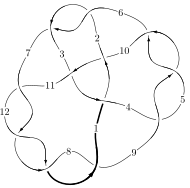
\includegraphics[width=112pt]{../../../GIT/diagram.site/Diagrams/png/1785_12a_0984.png}\\
\ \ \ A knot diagram\footnotemark}&
\allowdisplaybreaks
\textbf{Linearized knot diagam} \\
\cline{2-2}
 &
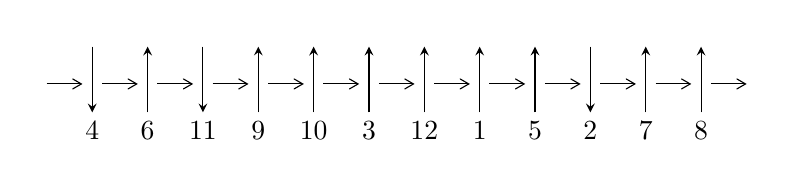
\begin{tikzpicture}[x=20pt, y=17pt]
	% nodes
	\node (C0) at (0, 0) {};
	\node (C1) at (1, 0) {};
	\node (C1U) at (1, +1) {};
	\node (C1D) at (1, -1) {4};

	\node (C2) at (2, 0) {};
	\node (C2U) at (2, +1) {};
	\node (C2D) at (2, -1) {6};

	\node (C3) at (3, 0) {};
	\node (C3U) at (3, +1) {};
	\node (C3D) at (3, -1) {11};

	\node (C4) at (4, 0) {};
	\node (C4U) at (4, +1) {};
	\node (C4D) at (4, -1) {9};

	\node (C5) at (5, 0) {};
	\node (C5U) at (5, +1) {};
	\node (C5D) at (5, -1) {10};

	\node (C6) at (6, 0) {};
	\node (C6U) at (6, +1) {};
	\node (C6D) at (6, -1) {3};

	\node (C7) at (7, 0) {};
	\node (C7U) at (7, +1) {};
	\node (C7D) at (7, -1) {12};

	\node (C8) at (8, 0) {};
	\node (C8U) at (8, +1) {};
	\node (C8D) at (8, -1) {1};

	\node (C9) at (9, 0) {};
	\node (C9U) at (9, +1) {};
	\node (C9D) at (9, -1) {5};

	\node (C10) at (10, 0) {};
	\node (C10U) at (10, +1) {};
	\node (C10D) at (10, -1) {2};

	\node (C11) at (11, 0) {};
	\node (C11U) at (11, +1) {};
	\node (C11D) at (11, -1) {7};

	\node (C12) at (12, 0) {};
	\node (C12U) at (12, +1) {};
	\node (C12D) at (12, -1) {8};
	\node (C13) at (13, 0) {};

	% arrows
	\draw[->,>={angle 60}]
	(C0) edge (C1) (C1) edge (C2) (C2) edge (C3) (C3) edge (C4) (C4) edge (C5) (C5) edge (C6) (C6) edge (C7) (C7) edge (C8) (C8) edge (C9) (C9) edge (C10) (C10) edge (C11) (C11) edge (C12) (C12) edge (C13) ;	\draw[->,>=stealth]
	(C1U) edge (C1D) (C2D) edge (C2U) (C3U) edge (C3D) (C4D) edge (C4U) (C5D) edge (C5U) (C6D) edge (C6U) (C7D) edge (C7U) (C8D) edge (C8U) (C9D) edge (C9U) (C10U) edge (C10D) (C11D) edge (C11U) (C12D) edge (C12U) ;
	\end{tikzpicture} \\
\hhline{~~} \\& 
\textbf{Solving Sequence} \\ \cline{2-2} 
 &
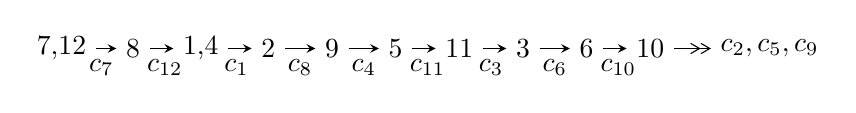
\begin{tikzpicture}[x=23pt, y=7pt]
	% node
	\node (A0) at (-1/8, 0) {7,12};
	\node (A1) at (1, 0) {8};
	\node (A2) at (33/16, 0) {1,4};
	\node (A3) at (25/8, 0) {2};
	\node (A4) at (33/8, 0) {9};
	\node (A5) at (41/8, 0) {5};
	\node (A6) at (49/8, 0) {11};
	\node (A7) at (57/8, 0) {3};
	\node (A8) at (65/8, 0) {6};
	\node (A9) at (73/8, 0) {10};
	\node (C1) at (1/2, -1) {$c_{7}$};
	\node (C2) at (3/2, -1) {$c_{12}$};
	\node (C3) at (21/8, -1) {$c_{1}$};
	\node (C4) at (29/8, -1) {$c_{8}$};
	\node (C5) at (37/8, -1) {$c_{4}$};
	\node (C6) at (45/8, -1) {$c_{11}$};
	\node (C7) at (53/8, -1) {$c_{3}$};
	\node (C8) at (61/8, -1) {$c_{6}$};
	\node (C9) at (69/8, -1) {$c_{10}$};
	\node (A10) at (11, 0) {$c_{2},c_{5},c_{9}$};

	% edge
	\draw[->,>=stealth]	
	(A0) edge (A1) (A1) edge (A2) (A2) edge (A3) (A3) edge (A4) (A4) edge (A5) (A5) edge (A6) (A6) edge (A7) (A7) edge (A8) (A8) edge (A9) ;
	\draw[->>,>={angle 60}]	
	(A9) edge (A10);
\end{tikzpicture} \\ 

\end{tabular} \\

\footnotetext{
The image of knot diagram is generated by the software ``\textbf{Draw programme}" developed by Andrew Bartholomew(\url{http://www.layer8.co.uk/maths/draw/index.htm\#Running-draw}), where we modified some parts for our purpose(\url{https://github.com/CATsTAILs/LinksPainter}).
}\phantom \\ \newline 
\centering \textbf{Ideals for irreducible components\footnotemark of $X_{\text{par}}$} 
 
\begin{align*}
I^u_{1}&=\langle 
-5.50090\times10^{58} u^{64}+1.26323\times10^{59} u^{63}+\cdots+2.01207\times10^{58} b-1.19889\times10^{59},\\
\phantom{I^u_{1}}&\phantom{= \langle  }-8.05777\times10^{57} u^{64}-9.65753\times10^{57} u^{63}+\cdots+2.01207\times10^{58} a+2.45376\times10^{59},\;u^{65}- u^{64}+\cdots+15 u+1\rangle \\
I^u_{2}&=\langle 
- u^{12}+8 u^{10}- u^9-24 u^8+6 u^7+34 u^6-12 u^5-24 u^4+9 u^3+8 u^2+b-2 u-1,\\
\phantom{I^u_{2}}&\phantom{= \langle  }u^{13}-10 u^{11}+2 u^{10}+39 u^9-15 u^8-74 u^7+40 u^6+70 u^5-46 u^4-31 u^3+24 u^2+a+5 u-6,\\
\phantom{I^u_{2}}&\phantom{= \langle  }u^{14}-10 u^{12}+u^{11}+39 u^{10}-8 u^9-75 u^8+23 u^7+75 u^6-29 u^5-39 u^4+17 u^3+10 u^2-5 u-1\rangle \\
\\
\end{align*}
\raggedright * 2 irreducible components of $\dim_{\mathbb{C}}=0$, with total 79 representations.\\
\footnotetext{All coefficients of polynomials are rational numbers. But the coefficients are sometimes approximated in decimal forms when there is not enough margin.}
\newpage
\renewcommand{\arraystretch}{1}
\centering \section*{I. $I^u_{1}= \langle -5.50\times10^{58} u^{64}+1.26\times10^{59} u^{63}+\cdots+2.01\times10^{58} b-1.20\times10^{59},\;-8.06\times10^{57} u^{64}-9.66\times10^{57} u^{63}+\cdots+2.01\times10^{58} a+2.45\times10^{59},\;u^{65}- u^{64}+\cdots+15 u+1 \rangle$}
\flushleft \textbf{(i) Arc colorings}\\
\begin{tabular}{m{7pt} m{180pt} m{7pt} m{180pt} }
\flushright $a_{7}=$&$\begin{pmatrix}1\\0\end{pmatrix}$ \\
\flushright $a_{12}=$&$\begin{pmatrix}0\\u\end{pmatrix}$ \\
\flushright $a_{8}=$&$\begin{pmatrix}1\\- u^2\end{pmatrix}$ \\
\flushright $a_{1}=$&$\begin{pmatrix}u\\- u^3+u\end{pmatrix}$ \\
\flushright $a_{4}=$&$\begin{pmatrix}0.400471 u^{64}+0.479979 u^{63}+\cdots-6.74840 u-12.1952\\2.73394 u^{64}-6.27826 u^{63}+\cdots+62.2065 u+5.95850\end{pmatrix}$ \\
\flushright $a_{2}=$&$\begin{pmatrix}-1.62795 u^{64}+0.503503 u^{63}+\cdots-247.503 u-7.75301\\1.78903 u^{64}-2.08762 u^{63}+\cdots+55.9693 u+3.12673\end{pmatrix}$ \\
\flushright $a_{9}=$&$\begin{pmatrix}- u^2+1\\u^4-2 u^2\end{pmatrix}$ \\
\flushright $a_{5}=$&$\begin{pmatrix}0.863498 u^{64}-0.649790 u^{63}+\cdots-2.52825 u-10.4084\\1.54027 u^{64}-4.04431 u^{63}+\cdots+38.9849 u+4.28279\end{pmatrix}$ \\
\flushright $a_{11}=$&$\begin{pmatrix}- u\\u\end{pmatrix}$ \\
\flushright $a_{3}=$&$\begin{pmatrix}1.78938 u^{64}-2.87215 u^{63}+\cdots+30.0752 u-9.53132\\1.34504 u^{64}-2.92613 u^{63}+\cdots+25.3829 u+3.29464\end{pmatrix}$ \\
\flushright $a_{6}=$&$\begin{pmatrix}0.633467 u^{64}+0.762597 u^{63}+\cdots+99.1976 u-8.80979\\-0.359097 u^{64}-0.374796 u^{63}+\cdots-20.0580 u+0.472607\end{pmatrix}$ \\
\flushright $a_{10}=$&$\begin{pmatrix}0.648781 u^{64}-2.39549 u^{63}+\cdots+0.850744 u+17.0104\\2.20379 u^{64}-2.48811 u^{63}+\cdots+37.1721 u+0.459690\end{pmatrix}$\\&\end{tabular}
\flushleft \textbf{(ii) Obstruction class $= -1$}\\~\\
\flushleft \textbf{(iii) Cusp Shapes $= 1.12410 u^{64}-3.19508 u^{63}+\cdots-2.97273 u+13.0445$}\\~\\
\newpage\renewcommand{\arraystretch}{1}
\flushleft \textbf{(iv) u-Polynomials at the component}\newline \\
\begin{tabular}{m{50pt}|m{274pt}}
Crossings & \hspace{64pt}u-Polynomials at each crossing \\
\hline $$\begin{aligned}c_{1}\end{aligned}$$&$\begin{aligned}
&u^{65}-10 u^{64}+\cdots-646157 u+15851
\end{aligned}$\\
\hline $$\begin{aligned}c_{2},c_{6}\end{aligned}$$&$\begin{aligned}
&u^{65}-31 u^{63}+\cdots+4 u+1
\end{aligned}$\\
\hline $$\begin{aligned}c_{3}\end{aligned}$$&$\begin{aligned}
&u^{65}-2 u^{64}+\cdots+1806 u-14929
\end{aligned}$\\
\hline $$\begin{aligned}c_{4},c_{5},c_{9}\end{aligned}$$&$\begin{aligned}
&u^{65}+2 u^{64}+\cdots+81 u-1
\end{aligned}$\\
\hline $$\begin{aligned}c_{7},c_{8},c_{11}\\c_{12}\end{aligned}$$&$\begin{aligned}
&u^{65}+u^{64}+\cdots+15 u-1
\end{aligned}$\\
\hline $$\begin{aligned}c_{10}\end{aligned}$$&$\begin{aligned}
&u^{65}+3 u^{64}+\cdots-18311 u+5039
\end{aligned}$\\
\hline
\end{tabular}\\~\\
\newpage\renewcommand{\arraystretch}{1}
\flushleft \textbf{(v) Riley Polynomials at the component}\newline \\
\begin{tabular}{m{50pt}|m{274pt}}
Crossings & \hspace{64pt}Riley Polynomials at each crossing \\
\hline $$\begin{aligned}c_{1}\end{aligned}$$&$\begin{aligned}
&y^{65}+42 y^{64}+\cdots+350419778635 y-251254201
\end{aligned}$\\
\hline $$\begin{aligned}c_{2},c_{6}\end{aligned}$$&$\begin{aligned}
&y^{65}-62 y^{64}+\cdots-446 y-1
\end{aligned}$\\
\hline $$\begin{aligned}c_{3}\end{aligned}$$&$\begin{aligned}
&y^{65}+34 y^{64}+\cdots+1425607182 y-222875041
\end{aligned}$\\
\hline $$\begin{aligned}c_{4},c_{5},c_{9}\end{aligned}$$&$\begin{aligned}
&y^{65}-74 y^{64}+\cdots+6515 y-1
\end{aligned}$\\
\hline $$\begin{aligned}c_{7},c_{8},c_{11}\\c_{12}\end{aligned}$$&$\begin{aligned}
&y^{65}-85 y^{64}+\cdots-125 y-1
\end{aligned}$\\
\hline $$\begin{aligned}c_{10}\end{aligned}$$&$\begin{aligned}
&y^{65}+27 y^{64}+\cdots+94761095 y-25391521
\end{aligned}$\\
\hline
\end{tabular}\\~\\
\newpage\flushleft \textbf{(vi) Complex Volumes and Cusp Shapes}
$$\begin{array}{c|c|c}  
\text{Solutions to }I^u_{1}& \I (\text{vol} + \sqrt{-1}CS) & \text{Cusp shape}\\
 \hline 
\begin{aligned}
u &= \phantom{-}0.889757 + 0.433062 I \\
a &= \phantom{-}0.595422 - 0.198986 I \\
b &= \phantom{-}0.281933 + 0.547527 I\end{aligned}
 & \phantom{-}7.58885 + 1.40904 I & \phantom{-0.000000 } 0 \\ \hline\begin{aligned}
u &= \phantom{-}0.889757 - 0.433062 I \\
a &= \phantom{-}0.595422 + 0.198986 I \\
b &= \phantom{-}0.281933 - 0.547527 I\end{aligned}
 & \phantom{-}7.58885 - 1.40904 I & \phantom{-0.000000 } 0 \\ \hline\begin{aligned}
u &= \phantom{-}0.935679 + 0.430142 I \\
a &= -0.133556 + 0.252790 I \\
b &= \phantom{-}0.002645 + 1.300830 I\end{aligned}
 & \phantom{-}5.78424 + 7.60090 I & \phantom{-0.000000 } 0 \\ \hline\begin{aligned}
u &= \phantom{-}0.935679 - 0.430142 I \\
a &= -0.133556 - 0.252790 I \\
b &= \phantom{-}0.002645 - 1.300830 I\end{aligned}
 & \phantom{-}5.78424 - 7.60090 I & \phantom{-0.000000 } 0 \\ \hline\begin{aligned}
u &= -0.868051 + 0.564459 I \\
a &= -0.220898 - 0.124404 I \\
b &= \phantom{-}0.568115 - 0.720158 I\end{aligned}
 & \phantom{-}4.84341 - 0.52476 I & \phantom{-0.000000 } 0 \\ \hline\begin{aligned}
u &= -0.868051 - 0.564459 I \\
a &= -0.220898 + 0.124404 I \\
b &= \phantom{-}0.568115 + 0.720158 I\end{aligned}
 & \phantom{-}4.84341 + 0.52476 I & \phantom{-0.000000 } 0 \\ \hline\begin{aligned}
u &= \phantom{-}0.157396 + 0.936252 I \\
a &= -0.718874 - 0.451433 I \\
b &= -0.314810 - 0.120327 I\end{aligned}
 & \phantom{-}9.74575 + 6.14975 I & \phantom{-0.000000 } 0 \\ \hline\begin{aligned}
u &= \phantom{-}0.157396 - 0.936252 I \\
a &= -0.718874 + 0.451433 I \\
b &= -0.314810 + 0.120327 I\end{aligned}
 & \phantom{-}9.74575 - 6.14975 I & \phantom{-0.000000 } 0 \\ \hline\begin{aligned}
u &= -0.866334 + 0.387041 I \\
a &= \phantom{-}0.177626 + 0.667924 I \\
b &= -0.38134 - 1.60962 I\end{aligned}
 & \phantom{-}7.62669 - 5.64553 I & \phantom{-0.000000 } 0 \\ \hline\begin{aligned}
u &= -0.866334 - 0.387041 I \\
a &= \phantom{-}0.177626 - 0.667924 I \\
b &= -0.38134 + 1.60962 I\end{aligned}
 & \phantom{-}7.62669 + 5.64553 I & \phantom{-0.000000 } 0\\
 \hline 
 \end{array}$$\newpage$$\begin{array}{c|c|c}  
\text{Solutions to }I^u_{1}& \I (\text{vol} + \sqrt{-1}CS) & \text{Cusp shape}\\
 \hline 
\begin{aligned}
u &= \phantom{-}0.936520 + 0.039908 I \\
a &= -1.58250 - 0.14580 I \\
b &= \phantom{-}0.084560 - 1.007070 I\end{aligned}
 & \phantom{-}11.75260 + 2.96607 I & \phantom{-0.000000 } 0 \\ \hline\begin{aligned}
u &= \phantom{-}0.936520 - 0.039908 I \\
a &= -1.58250 + 0.14580 I \\
b &= \phantom{-}0.084560 + 1.007070 I\end{aligned}
 & \phantom{-}11.75260 - 2.96607 I & \phantom{-0.000000 } 0 \\ \hline\begin{aligned}
u &= -0.891446 + 0.041272 I \\
a &= -1.76473 - 0.50188 I \\
b &= \phantom{-}1.41399 + 1.40674 I\end{aligned}
 & \phantom{-}11.30310 + 2.13802 I & \phantom{-}18.7856 - 3.2914 I \\ \hline\begin{aligned}
u &= -0.891446 - 0.041272 I \\
a &= -1.76473 + 0.50188 I \\
b &= \phantom{-}1.41399 - 1.40674 I\end{aligned}
 & \phantom{-}11.30310 - 2.13802 I & \phantom{-}18.7856 + 3.2914 I \\ \hline\begin{aligned}
u &= -0.863593 + 0.206273 I \\
a &= \phantom{-}0.735499 + 0.727785 I \\
b &= -0.004341 + 1.321520 I\end{aligned}
 & \phantom{-}4.72318 - 1.99911 I & \phantom{-}16.8500 + 4.6466 I \\ \hline\begin{aligned}
u &= -0.863593 - 0.206273 I \\
a &= \phantom{-}0.735499 - 0.727785 I \\
b &= -0.004341 - 1.321520 I\end{aligned}
 & \phantom{-}4.72318 + 1.99911 I & \phantom{-}16.8500 - 4.6466 I \\ \hline\begin{aligned}
u &= \phantom{-}0.825189 + 0.164350 I \\
a &= \phantom{-}1.109760 - 0.001937 I \\
b &= -0.97431 - 1.02822 I\end{aligned}
 & \phantom{-}4.60530 + 1.62841 I & \phantom{-}19.0869 - 5.0351 I \\ \hline\begin{aligned}
u &= \phantom{-}0.825189 - 0.164350 I \\
a &= \phantom{-}1.109760 + 0.001937 I \\
b &= -0.97431 + 1.02822 I\end{aligned}
 & \phantom{-}4.60530 - 1.62841 I & \phantom{-}19.0869 + 5.0351 I \\ \hline\begin{aligned}
u &= \phantom{-}0.782280 + 0.256564 I \\
a &= -0.067172 + 0.264192 I \\
b &= \phantom{-}0.419229 - 1.239770 I\end{aligned}
 & \phantom{-}1.05736 + 3.42824 I & \phantom{-}9.38737 - 8.82437 I \\ \hline\begin{aligned}
u &= \phantom{-}0.782280 - 0.256564 I \\
a &= -0.067172 - 0.264192 I \\
b &= \phantom{-}0.419229 + 1.239770 I\end{aligned}
 & \phantom{-}1.05736 - 3.42824 I & \phantom{-}9.38737 + 8.82437 I\\
 \hline 
 \end{array}$$\newpage$$\begin{array}{c|c|c}  
\text{Solutions to }I^u_{1}& \I (\text{vol} + \sqrt{-1}CS) & \text{Cusp shape}\\
 \hline 
\begin{aligned}
u &= -1.049540 + 0.559169 I \\
a &= -0.0045583 - 0.0656234 I \\
b &= \phantom{-}0.073399 + 1.340640 I\end{aligned}
 & \phantom{-}13.4741 - 11.0913 I & \phantom{-0.000000 } 0 \\ \hline\begin{aligned}
u &= -1.049540 - 0.559169 I \\
a &= -0.0045583 + 0.0656234 I \\
b &= \phantom{-}0.073399 - 1.340640 I\end{aligned}
 & \phantom{-}13.4741 + 11.0913 I & \phantom{-0.000000 } 0 \\ \hline\begin{aligned}
u &= -1.22679\phantom{ +0.000000I} \\
a &= -0.270827\phantom{ +0.000000I} \\
b &= -0.374892\phantom{ +0.000000I}\end{aligned}
 & \phantom{-}2.39981\phantom{ +0.000000I} & \phantom{-0.000000 } 0 \\ \hline\begin{aligned}
u &= \phantom{-}0.952627 + 0.791056 I \\
a &= -0.0432079 + 0.0247757 I \\
b &= -0.402011 - 0.728715 I\end{aligned}
 & \phantom{-}12.00730 - 0.38636 I & \phantom{-0.000000 } 0 \\ \hline\begin{aligned}
u &= \phantom{-}0.952627 - 0.791056 I \\
a &= -0.0432079 - 0.0247757 I \\
b &= -0.402011 + 0.728715 I\end{aligned}
 & \phantom{-}12.00730 + 0.38636 I & \phantom{-0.000000 } 0 \\ \hline\begin{aligned}
u &= -0.096388 + 0.710673 I \\
a &= \phantom{-}0.837011 - 0.685506 I \\
b &= \phantom{-}0.488500 - 0.029172 I\end{aligned}
 & \phantom{-}2.61549 - 3.79888 I & \phantom{-}9.89337 + 6.78663 I \\ \hline\begin{aligned}
u &= -0.096388 - 0.710673 I \\
a &= \phantom{-}0.837011 + 0.685506 I \\
b &= \phantom{-}0.488500 + 0.029172 I\end{aligned}
 & \phantom{-}2.61549 + 3.79888 I & \phantom{-}9.89337 - 6.78663 I \\ \hline\begin{aligned}
u &= -0.706625 + 0.004243 I \\
a &= -0.326615 + 0.075243 I \\
b &= -0.438772 + 0.728388 I\end{aligned}
 & \phantom{-}1.114370 + 0.096093 I & \phantom{-}9.80971 + 0.48102 I \\ \hline\begin{aligned}
u &= -0.706625 - 0.004243 I \\
a &= -0.326615 - 0.075243 I \\
b &= -0.438772 - 0.728388 I\end{aligned}
 & \phantom{-}1.114370 - 0.096093 I & \phantom{-}9.80971 - 0.48102 I \\ \hline\begin{aligned}
u &= \phantom{-}1.30205\phantom{ +0.000000I} \\
a &= \phantom{-}0.756337\phantom{ +0.000000I} \\
b &= -0.949659\phantom{ +0.000000I}\end{aligned}
 & \phantom{-}5.71531\phantom{ +0.000000I} & \phantom{-0.000000 } 0\\
 \hline 
 \end{array}$$\newpage$$\begin{array}{c|c|c}  
\text{Solutions to }I^u_{1}& \I (\text{vol} + \sqrt{-1}CS) & \text{Cusp shape}\\
 \hline 
\begin{aligned}
u &= \phantom{-}0.011225 + 0.631699 I \\
a &= \phantom{-}1.173430 + 0.684067 I \\
b &= -0.243702 + 0.396416 I\end{aligned}
 & \phantom{-}4.95418 + 2.21427 I & \phantom{-}8.45324 - 3.11503 I \\ \hline\begin{aligned}
u &= \phantom{-}0.011225 - 0.631699 I \\
a &= \phantom{-}1.173430 - 0.684067 I \\
b &= -0.243702 - 0.396416 I\end{aligned}
 & \phantom{-}4.95418 - 2.21427 I & \phantom{-}8.45324 + 3.11503 I \\ \hline\begin{aligned}
u &= \phantom{-}1.46845\phantom{ +0.000000I} \\
a &= -0.187024\phantom{ +0.000000I} \\
b &= \phantom{-}1.14204\phantom{ +0.000000I}\end{aligned}
 & \phantom{-}6.49904\phantom{ +0.000000I} & \phantom{-0.000000 } 0 \\ \hline\begin{aligned}
u &= -0.414265\phantom{ +0.000000I} \\
a &= \phantom{-}3.15526\phantom{ +0.000000I} \\
b &= -0.0379566\phantom{ +0.000000I}\end{aligned}
 & \phantom{-}0.0573235\phantom{ +0.000000I} & \phantom{-}19.4200\phantom{ +0.000000I} \\ \hline\begin{aligned}
u &= \phantom{-}0.050717 + 0.407384 I \\
a &= -0.98626 + 1.37309 I \\
b &= \phantom{-}0.106234 + 0.222035 I\end{aligned}
 & -1.10170 - 1.06626 I & -0.72797 + 3.75877 I \\ \hline\begin{aligned}
u &= \phantom{-}0.050717 - 0.407384 I \\
a &= -0.98626 - 1.37309 I \\
b &= \phantom{-}0.106234 - 0.222035 I\end{aligned}
 & -1.10170 + 1.06626 I & -0.72797 - 3.75877 I \\ \hline\begin{aligned}
u &= -0.002304 + 0.351380 I \\
a &= -1.95027 - 1.37104 I \\
b &= -0.824432 + 0.186984 I\end{aligned}
 & \phantom{-}2.13526 + 0.06396 I & \phantom{-}7.70510 + 0.30032 I \\ \hline\begin{aligned}
u &= -0.002304 - 0.351380 I \\
a &= -1.95027 + 1.37104 I \\
b &= -0.824432 - 0.186984 I\end{aligned}
 & \phantom{-}2.13526 - 0.06396 I & \phantom{-}7.70510 - 0.30032 I \\ \hline\begin{aligned}
u &= -0.350174\phantom{ +0.000000I} \\
a &= -0.614828\phantom{ +0.000000I} \\
b &= -0.463481\phantom{ +0.000000I}\end{aligned}
 & \phantom{-}0.719899\phantom{ +0.000000I} & \phantom{-}14.9890\phantom{ +0.000000I} \\ \hline\begin{aligned}
u &= \phantom{-}1.65272 + 0.01145 I \\
a &= \phantom{-}0.47953 + 1.86610 I \\
b &= -0.77556 - 2.58159 I\end{aligned}
 & \phantom{-}9.51546 + 0.03244 I & \phantom{-0.000000 } 0\\
 \hline 
 \end{array}$$\newpage$$\begin{array}{c|c|c}  
\text{Solutions to }I^u_{1}& \I (\text{vol} + \sqrt{-1}CS) & \text{Cusp shape}\\
 \hline 
\begin{aligned}
u &= \phantom{-}1.65272 - 0.01145 I \\
a &= \phantom{-}0.47953 - 1.86610 I \\
b &= -0.77556 + 2.58159 I\end{aligned}
 & \phantom{-}9.51546 - 0.03244 I & \phantom{-0.000000 } 0 \\ \hline\begin{aligned}
u &= -1.65709 + 0.05434 I \\
a &= -0.25689 - 2.19662 I \\
b &= \phantom{-}0.48205 + 2.85246 I\end{aligned}
 & \phantom{-}9.61848 - 4.52679 I & \phantom{-0.000000 } 0 \\ \hline\begin{aligned}
u &= -1.65709 - 0.05434 I \\
a &= -0.25689 + 2.19662 I \\
b &= \phantom{-}0.48205 - 2.85246 I\end{aligned}
 & \phantom{-}9.61848 + 4.52679 I & \phantom{-0.000000 } 0 \\ \hline\begin{aligned}
u &= -1.66991 + 0.04242 I \\
a &= \phantom{-}0.76197 - 1.61866 I \\
b &= -0.36741 + 2.21521 I\end{aligned}
 & \phantom{-}13.41440 - 2.40644 I & \phantom{-0.000000 } 0 \\ \hline\begin{aligned}
u &= -1.66991 - 0.04242 I \\
a &= \phantom{-}0.76197 + 1.61866 I \\
b &= -0.36741 - 2.21521 I\end{aligned}
 & \phantom{-}13.41440 + 2.40644 I & \phantom{-0.000000 } 0 \\ \hline\begin{aligned}
u &= \phantom{-}1.67767 + 0.09570 I \\
a &= \phantom{-}0.05955 - 2.48218 I \\
b &= -0.26406 + 3.07470 I\end{aligned}
 & \phantom{-}16.5146 + 7.4665 I & \phantom{-0.000000 } 0 \\ \hline\begin{aligned}
u &= \phantom{-}1.67767 - 0.09570 I \\
a &= \phantom{-}0.05955 + 2.48218 I \\
b &= -0.26406 - 3.07470 I\end{aligned}
 & \phantom{-}16.5146 - 7.4665 I & \phantom{-0.000000 } 0 \\ \hline\begin{aligned}
u &= \phantom{-}1.68402 + 0.05115 I \\
a &= -0.52918 + 2.34990 I \\
b &= \phantom{-}1.42152 - 3.59158 I\end{aligned}
 & \phantom{-}13.74990 + 2.97652 I & \phantom{-0.000000 } 0 \\ \hline\begin{aligned}
u &= \phantom{-}1.68402 - 0.05115 I \\
a &= -0.52918 - 2.34990 I \\
b &= \phantom{-}1.42152 + 3.59158 I\end{aligned}
 & \phantom{-}13.74990 - 2.97652 I & \phantom{-0.000000 } 0 \\ \hline\begin{aligned}
u &= \phantom{-}1.69185 + 0.00973 I \\
a &= -1.06345 + 1.76949 I \\
b &= \phantom{-}0.64856 - 2.29976 I\end{aligned}
 & -18.9704 - 1.9445 I & \phantom{-0.000000 } 0\\
 \hline 
 \end{array}$$\newpage$$\begin{array}{c|c|c}  
\text{Solutions to }I^u_{1}& \I (\text{vol} + \sqrt{-1}CS) & \text{Cusp shape}\\
 \hline 
\begin{aligned}
u &= \phantom{-}1.69185 - 0.00973 I \\
a &= -1.06345 - 1.76949 I \\
b &= \phantom{-}0.64856 + 2.29976 I\end{aligned}
 & -18.9704 + 1.9445 I & \phantom{-0.000000 } 0 \\ \hline\begin{aligned}
u &= -1.69453 + 0.10643 I \\
a &= -0.47342 + 1.38437 I \\
b &= \phantom{-}0.84199 - 2.02585 I\end{aligned}
 & \phantom{-}16.6703 - 3.4851 I & \phantom{-0.000000 } 0 \\ \hline\begin{aligned}
u &= -1.69453 - 0.10643 I \\
a &= -0.47342 - 1.38437 I \\
b &= \phantom{-}0.84199 + 2.02585 I\end{aligned}
 & \phantom{-}16.6703 + 3.4851 I & \phantom{-0.000000 } 0 \\ \hline\begin{aligned}
u &= -1.69423 + 0.11190 I \\
a &= \phantom{-}0.06318 + 2.21599 I \\
b &= -0.64443 - 3.30761 I\end{aligned}
 & \phantom{-}14.9626 - 9.7162 I & \phantom{-0.000000 } 0 \\ \hline\begin{aligned}
u &= -1.69423 - 0.11190 I \\
a &= \phantom{-}0.06318 - 2.21599 I \\
b &= -0.64443 + 3.30761 I\end{aligned}
 & \phantom{-}14.9626 + 9.7162 I & \phantom{-0.000000 } 0 \\ \hline\begin{aligned}
u &= \phantom{-}1.69496 + 0.13798 I \\
a &= -0.387962 - 1.341050 I \\
b &= \phantom{-}0.04223 + 2.01775 I\end{aligned}
 & \phantom{-}13.8035 + 3.2283 I & \phantom{-0.000000 } 0 \\ \hline\begin{aligned}
u &= \phantom{-}1.69496 - 0.13798 I \\
a &= -0.387962 + 1.341050 I \\
b &= \phantom{-}0.04223 - 2.01775 I\end{aligned}
 & \phantom{-}13.8035 - 3.2283 I & \phantom{-0.000000 } 0 \\ \hline\begin{aligned}
u &= -1.70249 + 0.00913 I \\
a &= \phantom{-}0.76510 - 1.62903 I \\
b &= -1.89492 + 2.45435 I\end{aligned}
 & -18.3078 - 3.1530 I & \phantom{-0.000000 } 0 \\ \hline\begin{aligned}
u &= -1.70249 - 0.00913 I \\
a &= \phantom{-}0.76510 + 1.62903 I \\
b &= -1.89492 - 2.45435 I\end{aligned}
 & -18.3078 + 3.1530 I & \phantom{-0.000000 } 0 \\ \hline\begin{aligned}
u &= \phantom{-}1.73019 + 0.15438 I \\
a &= \phantom{-}0.02330 + 2.05733 I \\
b &= \phantom{-}0.51225 - 3.00877 I\end{aligned}
 & -16.3366 + 14.0024 I & \phantom{-0.000000 } 0\\
 \hline 
 \end{array}$$\newpage$$\begin{array}{c|c|c}  
\text{Solutions to }I^u_{1}& \I (\text{vol} + \sqrt{-1}CS) & \text{Cusp shape}\\
 \hline 
\begin{aligned}
u &= \phantom{-}1.73019 - 0.15438 I \\
a &= \phantom{-}0.02330 - 2.05733 I \\
b &= \phantom{-}0.51225 + 3.00877 I\end{aligned}
 & -16.3366 - 14.0024 I & \phantom{-0.000000 } 0 \\ \hline\begin{aligned}
u &= -1.75668 + 0.21779 I \\
a &= \phantom{-}0.222757 - 1.210750 I \\
b &= \phantom{-}0.07750 + 1.91022 I\end{aligned}
 & -18.1051 - 3.7291 I & \phantom{-0.000000 } 0 \\ \hline\begin{aligned}
u &= -1.75668 - 0.21779 I \\
a &= \phantom{-}0.222757 + 1.210750 I \\
b &= \phantom{-}0.07750 - 1.91022 I\end{aligned}
 & -18.1051 + 3.7291 I & \phantom{-0.000000 } 0 \\ \hline\begin{aligned}
u &= -0.0432217 + 0.0807555 I \\
a &= -11.91410 - 0.09743 I \\
b &= \phantom{-}1.40737 - 0.33426 I\end{aligned}
 & \phantom{-}8.63685 - 2.55255 I & \phantom{-}12.94052 - 1.53049 I \\ \hline\begin{aligned}
u &= -0.0432217 - 0.0807555 I \\
a &= -11.91410 + 0.09743 I \\
b &= \phantom{-}1.40737 + 0.33426 I\end{aligned}
 & \phantom{-}8.63685 + 2.55255 I & \phantom{-}12.94052 + 1.53049 I\\
 \hline 
 \end{array}$$\newpage\newpage\renewcommand{\arraystretch}{1}
\centering \section*{II. $I^u_{2}= \langle - u^{12}+8 u^{10}+\cdots+b-1,\;u^{13}-10 u^{11}+\cdots+a-6,\;u^{14}-10 u^{12}+\cdots-5 u-1 \rangle$}
\flushleft \textbf{(i) Arc colorings}\\
\begin{tabular}{m{7pt} m{180pt} m{7pt} m{180pt} }
\flushright $a_{7}=$&$\begin{pmatrix}1\\0\end{pmatrix}$ \\
\flushright $a_{12}=$&$\begin{pmatrix}0\\u\end{pmatrix}$ \\
\flushright $a_{8}=$&$\begin{pmatrix}1\\- u^2\end{pmatrix}$ \\
\flushright $a_{1}=$&$\begin{pmatrix}u\\- u^3+u\end{pmatrix}$ \\
\flushright $a_{4}=$&$\begin{pmatrix}- u^{13}+10 u^{11}+\cdots-5 u+6\\u^{12}-8 u^{10}+\cdots+2 u+1\end{pmatrix}$ \\
\flushright $a_{2}=$&$\begin{pmatrix}- u^{13}+10 u^{11}+\cdots-5 u+5\\- u^9+6 u^7-12 u^5+9 u^3-2 u\end{pmatrix}$ \\
\flushright $a_{9}=$&$\begin{pmatrix}- u^2+1\\u^4-2 u^2\end{pmatrix}$ \\
\flushright $a_{5}=$&$\begin{pmatrix}- u^{13}+u^{12}+\cdots-5 u+7\\u^{11}-7 u^9+17 u^7-17 u^5+8 u^3-3 u\end{pmatrix}$ \\
\flushright $a_{11}=$&$\begin{pmatrix}- u\\u\end{pmatrix}$ \\
\flushright $a_{3}=$&$\begin{pmatrix}- u^{13}+u^{12}+\cdots- u+7\\u^3-2 u\end{pmatrix}$ \\
\flushright $a_{6}=$&$\begin{pmatrix}- u^{13}+10 u^{11}+\cdots-3 u+3\\u^6-4 u^4+4 u^2\end{pmatrix}$ \\
\flushright $a_{10}=$&$\begin{pmatrix}- u^{11}+u^{10}+\cdots+u-5\\u^{13}-9 u^{11}+31 u^9-51 u^7+41 u^5-15 u^3+3 u\end{pmatrix}$\\&\end{tabular}
\flushleft \textbf{(ii) Obstruction class $= 1$}\\~\\
\flushleft \textbf{(iii) Cusp Shapes $= 3 u^{13}- u^{12}-31 u^{11}+12 u^{10}+123 u^9-54 u^8-234 u^7+113 u^6+222 u^5-112 u^4-107 u^3+53 u^2+23 u$}\\~\\
\newpage\renewcommand{\arraystretch}{1}
\flushleft \textbf{(iv) u-Polynomials at the component}\newline \\
\begin{tabular}{m{50pt}|m{274pt}}
Crossings & \hspace{64pt}u-Polynomials at each crossing \\
\hline $$\begin{aligned}c_{1}\end{aligned}$$&$\begin{aligned}
&u^{14}+3 u^{13}+\cdots- u-1
\end{aligned}$\\
\hline $$\begin{aligned}c_{2}\end{aligned}$$&$\begin{aligned}
&u^{14}-3 u^{13}+\cdots-4 u+1
\end{aligned}$\\
\hline $$\begin{aligned}c_{3}\end{aligned}$$&$\begin{aligned}
&u^{14}+u^{13}+\cdots-2 u+1
\end{aligned}$\\
\hline $$\begin{aligned}c_{4},c_{5}\end{aligned}$$&$\begin{aligned}
&u^{14}+u^{13}+\cdots+u-1
\end{aligned}$\\
\hline $$\begin{aligned}c_{6}\end{aligned}$$&$\begin{aligned}
&u^{14}+3 u^{13}+\cdots+4 u+1
\end{aligned}$\\
\hline $$\begin{aligned}c_{7},c_{8}\end{aligned}$$&$\begin{aligned}
&u^{14}-10 u^{12}+\cdots-5 u-1
\end{aligned}$\\
\hline $$\begin{aligned}c_{9}\end{aligned}$$&$\begin{aligned}
&u^{14}- u^{13}+\cdots- u-1
\end{aligned}$\\
\hline $$\begin{aligned}c_{10}\end{aligned}$$&$\begin{aligned}
&u^{14}+2 u^{13}+\cdots- u+1
\end{aligned}$\\
\hline $$\begin{aligned}c_{11},c_{12}\end{aligned}$$&$\begin{aligned}
&u^{14}-10 u^{12}+\cdots+5 u-1
\end{aligned}$\\
\hline
\end{tabular}\\~\\
\newpage\renewcommand{\arraystretch}{1}
\flushleft \textbf{(v) Riley Polynomials at the component}\newline \\
\begin{tabular}{m{50pt}|m{274pt}}
Crossings & \hspace{64pt}Riley Polynomials at each crossing \\
\hline $$\begin{aligned}c_{1}\end{aligned}$$&$\begin{aligned}
&y^{14}+3 y^{13}+\cdots-9 y+1
\end{aligned}$\\
\hline $$\begin{aligned}c_{2},c_{6}\end{aligned}$$&$\begin{aligned}
&y^{14}-17 y^{13}+\cdots-60 y+1
\end{aligned}$\\
\hline $$\begin{aligned}c_{3}\end{aligned}$$&$\begin{aligned}
&y^{14}+3 y^{13}+\cdots+4 y^3+1
\end{aligned}$\\
\hline $$\begin{aligned}c_{4},c_{5},c_{9}\end{aligned}$$&$\begin{aligned}
&y^{14}-17 y^{13}+\cdots- y+1
\end{aligned}$\\
\hline $$\begin{aligned}c_{7},c_{8},c_{11}\\c_{12}\end{aligned}$$&$\begin{aligned}
&y^{14}-20 y^{13}+\cdots-45 y+1
\end{aligned}$\\
\hline $$\begin{aligned}c_{10}\end{aligned}$$&$\begin{aligned}
&y^{14}+4 y^{11}+\cdots+3 y+1
\end{aligned}$\\
\hline
\end{tabular}\\~\\
\newpage\flushleft \textbf{(vi) Complex Volumes and Cusp Shapes}
$$\begin{array}{c|c|c}  
\text{Solutions to }I^u_{2}& \I (\text{vol} + \sqrt{-1}CS) & \text{Cusp shape}\\
 \hline 
\begin{aligned}
u &= \phantom{-}0.968017 + 0.337938 I \\
a &= \phantom{-}1.078150 - 0.571014 I \\
b &= -0.709305 + 0.039438 I\end{aligned}
 & \phantom{-}10.20040 - 0.82211 I & \phantom{-}14.2370 - 0.6203 I \\ \hline\begin{aligned}
u &= \phantom{-}0.968017 - 0.337938 I \\
a &= \phantom{-}1.078150 + 0.571014 I \\
b &= -0.709305 - 0.039438 I\end{aligned}
 & \phantom{-}10.20040 + 0.82211 I & \phantom{-}14.2370 + 0.6203 I \\ \hline\begin{aligned}
u &= -1.14545\phantom{ +0.000000I} \\
a &= -0.563709\phantom{ +0.000000I} \\
b &= -0.155012\phantom{ +0.000000I}\end{aligned}
 & \phantom{-}2.82868\phantom{ +0.000000I} & \phantom{-}18.6140\phantom{ +0.000000I} \\ \hline\begin{aligned}
u &= -0.720462 + 0.270481 I \\
a &= -0.628432 - 0.675348 I \\
b &= \phantom{-}0.656755 - 0.815273 I\end{aligned}
 & \phantom{-}3.73792 - 1.01626 I & \phantom{-}11.08062 + 0.61543 I \\ \hline\begin{aligned}
u &= -0.720462 - 0.270481 I \\
a &= -0.628432 + 0.675348 I \\
b &= \phantom{-}0.656755 + 0.815273 I\end{aligned}
 & \phantom{-}3.73792 + 1.01626 I & \phantom{-}11.08062 - 0.61543 I \\ \hline\begin{aligned}
u &= \phantom{-}0.558487 + 0.398529 I \\
a &= \phantom{-}0.112815 + 0.298362 I \\
b &= -1.03491 - 1.00628 I\end{aligned}
 & \phantom{-}8.88600 + 3.51593 I & \phantom{-}15.2342 - 5.4123 I \\ \hline\begin{aligned}
u &= \phantom{-}0.558487 - 0.398529 I \\
a &= \phantom{-}0.112815 - 0.298362 I \\
b &= -1.03491 + 1.00628 I\end{aligned}
 & \phantom{-}8.88600 - 3.51593 I & \phantom{-}15.2342 + 5.4123 I \\ \hline\begin{aligned}
u &= \phantom{-}1.37496\phantom{ +0.000000I} \\
a &= -0.439623\phantom{ +0.000000I} \\
b &= \phantom{-}1.10231\phantom{ +0.000000I}\end{aligned}
 & \phantom{-}4.87233\phantom{ +0.000000I} & \phantom{-}7.57420\phantom{ +0.000000I} \\ \hline\begin{aligned}
u &= -1.64578 + 0.11762 I \\
a &= \phantom{-}0.89070 - 1.83826 I \\
b &= -0.91793 + 2.49252 I\end{aligned}
 & \phantom{-}16.7686 - 5.4927 I & \phantom{-}16.7104 + 3.4526 I \\ \hline\begin{aligned}
u &= -1.64578 - 0.11762 I \\
a &= \phantom{-}0.89070 + 1.83826 I \\
b &= -0.91793 - 2.49252 I\end{aligned}
 & \phantom{-}16.7686 + 5.4927 I & \phantom{-}16.7104 - 3.4526 I\\
 \hline 
 \end{array}$$\newpage$$\begin{array}{c|c|c}  
\text{Solutions to }I^u_{2}& \I (\text{vol} + \sqrt{-1}CS) & \text{Cusp shape}\\
 \hline 
\begin{aligned}
u &= \phantom{-}1.66941 + 0.05921 I \\
a &= -0.19583 - 1.71092 I \\
b &= -0.33171 + 2.51769 I\end{aligned}
 & \phantom{-}12.32760 + 2.20627 I & \phantom{-}11.06041 - 0.00050 I \\ \hline\begin{aligned}
u &= \phantom{-}1.66941 - 0.05921 I \\
a &= -0.19583 + 1.71092 I \\
b &= -0.33171 - 2.51769 I\end{aligned}
 & \phantom{-}12.32760 - 2.20627 I & \phantom{-}11.06041 + 0.00050 I \\ \hline\begin{aligned}
u &= -1.72337\phantom{ +0.000000I} \\
a &= \phantom{-}0.416712\phantom{ +0.000000I} \\
b &= \phantom{-}0.220318\phantom{ +0.000000I}\end{aligned}
 & -19.0939\phantom{ +0.000000I} & \phantom{-}17.1450\phantom{ +0.000000I} \\ \hline\begin{aligned}
u &= -0.165484\phantom{ +0.000000I} \\
a &= \phantom{-}6.07182\phantom{ +0.000000I} \\
b &= \phantom{-}0.506584\phantom{ +0.000000I}\end{aligned}
 & -0.331903\phantom{ +0.000000I} & -1.97830\phantom{ +0.000000I}\\
 \hline 
 \end{array}$$\newpage
\newpage\renewcommand{\arraystretch}{1}
\centering \section*{ III. u-Polynomials}
\begin{tabular}{m{50pt}|m{274pt}}
Crossings & \hspace{64pt}u-Polynomials at each crossing \\
\hline $$\begin{aligned}c_{1}\end{aligned}$$&$\begin{aligned}
&(u^{14}+3 u^{13}+\cdots- u-1)(u^{65}-10 u^{64}+\cdots-646157 u+15851)
\end{aligned}$\\
\hline $$\begin{aligned}c_{2}\end{aligned}$$&$\begin{aligned}
&(u^{14}-3 u^{13}+\cdots-4 u+1)(u^{65}-31 u^{63}+\cdots+4 u+1)
\end{aligned}$\\
\hline $$\begin{aligned}c_{3}\end{aligned}$$&$\begin{aligned}
&(u^{14}+u^{13}+\cdots-2 u+1)(u^{65}-2 u^{64}+\cdots+1806 u-14929)
\end{aligned}$\\
\hline $$\begin{aligned}c_{4},c_{5}\end{aligned}$$&$\begin{aligned}
&(u^{14}+u^{13}+\cdots+u-1)(u^{65}+2 u^{64}+\cdots+81 u-1)
\end{aligned}$\\
\hline $$\begin{aligned}c_{6}\end{aligned}$$&$\begin{aligned}
&(u^{14}+3 u^{13}+\cdots+4 u+1)(u^{65}-31 u^{63}+\cdots+4 u+1)
\end{aligned}$\\
\hline $$\begin{aligned}c_{7},c_{8}\end{aligned}$$&$\begin{aligned}
&(u^{14}-10 u^{12}+\cdots-5 u-1)(u^{65}+u^{64}+\cdots+15 u-1)
\end{aligned}$\\
\hline $$\begin{aligned}c_{9}\end{aligned}$$&$\begin{aligned}
&(u^{14}- u^{13}+\cdots- u-1)(u^{65}+2 u^{64}+\cdots+81 u-1)
\end{aligned}$\\
\hline $$\begin{aligned}c_{10}\end{aligned}$$&$\begin{aligned}
&(u^{14}+2 u^{13}+\cdots- u+1)(u^{65}+3 u^{64}+\cdots-18311 u+5039)
\end{aligned}$\\
\hline $$\begin{aligned}c_{11},c_{12}\end{aligned}$$&$\begin{aligned}
&(u^{14}-10 u^{12}+\cdots+5 u-1)(u^{65}+u^{64}+\cdots+15 u-1)
\end{aligned}$\\
\hline
\end{tabular}\newpage\renewcommand{\arraystretch}{1}
\centering \section*{ IV. Riley Polynomials}
\begin{tabular}{m{50pt}|m{274pt}}
Crossings & \hspace{64pt}Riley Polynomials at each crossing \\
\hline $$\begin{aligned}c_{1}\end{aligned}$$&$\begin{aligned}
&(y^{14}+3 y^{13}+\cdots-9 y+1)\\
&\cdot(y^{65}+42 y^{64}+\cdots+350419778635 y-251254201)
\end{aligned}$\\
\hline $$\begin{aligned}c_{2},c_{6}\end{aligned}$$&$\begin{aligned}
&(y^{14}-17 y^{13}+\cdots-60 y+1)(y^{65}-62 y^{64}+\cdots-446 y-1)
\end{aligned}$\\
\hline $$\begin{aligned}c_{3}\end{aligned}$$&$\begin{aligned}
&(y^{14}+3 y^{13}+\cdots+4 y^3+1)\\
&\cdot(y^{65}+34 y^{64}+\cdots+1425607182 y-222875041)
\end{aligned}$\\
\hline $$\begin{aligned}c_{4},c_{5},c_{9}\end{aligned}$$&$\begin{aligned}
&(y^{14}-17 y^{13}+\cdots- y+1)(y^{65}-74 y^{64}+\cdots+6515 y-1)
\end{aligned}$\\
\hline $$\begin{aligned}c_{7},c_{8},c_{11}\\c_{12}\end{aligned}$$&$\begin{aligned}
&(y^{14}-20 y^{13}+\cdots-45 y+1)(y^{65}-85 y^{64}+\cdots-125 y-1)
\end{aligned}$\\
\hline $$\begin{aligned}c_{10}\end{aligned}$$&$\begin{aligned}
&(y^{14}+4 y^{11}+\cdots+3 y+1)\\
&\cdot(y^{65}+27 y^{64}+\cdots+94761095 y-25391521)
\end{aligned}$\\
\hline
\end{tabular}
\vskip 2pc
\end{document}